\documentclass{report}
\usepackage[english]{babel}
\usepackage[utf8x]{inputenc}
\usepackage{amsmath}
\usepackage{graphicx}
\usepackage[colorinlistoftodos]{todonotes}
\usepackage{enumitem}
\usepackage{listings}
\usepackage{verbatim}
\usepackage{eurosym}
\usepackage[export]{adjustbox}
\usepackage{amssymb}
\usepackage{bussproofs}
\usepackage{amsmath}
\usepackage{tikz}
\usepackage{xcolor}
\usepackage{listings}
\usepackage{titletoc}
\usepackage{hyperref}

\hypersetup{
  colorlinks=true,
  linkcolor=black,
  urlcolor=blue,
  citecolor=black
}

\newcommand{\coverPage}[6]{%
%----------------------------------------------------------------------------------------
%	COVER START
%----------------------------------------------------------------------------------------
\begin{titlepage}

    \newcommand{\HRule}{\rule{\linewidth}{0.5mm}}
    \newcommand{\department}{#1}
    \newcommand{\course}{#2}
    \newcommand{\titleValue}{#3}
    \newcommand{\subtitleValue}{#4}
    \newcommand{\authorName}{#5}

    \center

    %----------------------------------------------------------------------------------------
    %	HEADER
    %----------------------------------------------------------------------------------------
    % 
\includegraphics{images/logo_usa.png}
    \vspace{0.5cm}
    \textsc{\Large \department}\\[0.5cm]
    \textsc{\Large \course}\\[0.5cm]
    \vfill

    %----------------------------------------------------------------------------------------
    %	TITLE
    %----------------------------------------------------------------------------------------

    \HRule\\
    \Huge
    \textbf{\titleValue}\\[0.5cm]
    \Large
    \textbf{\subtitleValue}\\
    \HRule\\[0.5cm]

    %----------------------------------------------------------------------------------------
    %	AUTHOR AND DATE
    %----------------------------------------------------------------------------------------

    \vfill
    \Large
    \textit{\authorName}\\
    {\large \today}\\[2cm]

\end{titlepage}
%----------------------------------------------------------------------------------------
%	COVER END
%----------------------------------------------------------------------------------------
}

\begin{document}
    % \coverPage{ Mathematics }{ Linear Algebra II }{ Diagonalization }{  }{ Alexander Mendoza }{\today}
    \tableofcontents
    \chapter{Some things to remember}
    \section{Determinants}
    We extend the definition of the determinant to $n \times n$ matrices for $n \geq 3$. For this definition, it is convenient to introduce the following notation: Given $A \in \mathrm{M}_{n \times n}(F)$, for $n \geq 2$, denote the $(n-1) \times(n-1)$ matrix obtained from $A$ by deleting row $i$ and column $j$ by $\bar{A}_{i j}$. Thus for
    $$
    A=\left(\begin{array}{lll}
    1 & 2 & 3 \\
    4 & 5 & 6 \\
    7 & 8 & 9
    \end{array}\right) \in \mathrm{M}_{3 \times 3}(R),
    $$
    we have
    $$
    \tilde{A}_{11}=\left(\begin{array}{ll}
    5 & 6 \\
    8 & 9
    \end{array}\right), \quad \tilde{A}_{13}=\left(\begin{array}{ll}
    4 & 5 \\
    7 & 8
    \end{array}\right), \quad \text { and } \quad \tilde{A}_{32}=\left(\begin{array}{ll}
    1 & 3 \\
    4 & 6
    \end{array}\right),
    $$
    and for
    $$
    B=\left(\begin{array}{rrrr}
    1 & -1 & 2 & -1 \\
    -3 & 4 & 1 & -1 \\
    2 & -5 & -3 & 8 \\
    -2 & 6 & -4 & 1
    \end{array}\right) \in \mathrm{M}_{4 \times 4}(R),
    $$
    we have
    $$
    \tilde{B}_{23}=\left(\begin{array}{rrr}
    1 & -1 & -1 \\
    2 & -5 & 8 \\
    -2 & 6 & 1
    \end{array}\right) \quad \text { and } \quad \tilde{B}_{42}=\left(\begin{array}{rrr}
    1 & 2 & -1 \\
    -3 & 1 & -1 \\
    2 & -3 & 8
    \end{array}\right) .
    $$

    \begin{defBox}
        Let $A \in \mathrm{M}_{n \times n}(F)$. If $n=1$, so that $A=\left(A_{11}\right)$, we define $\operatorname{det}(A)=A_{11}$. For $n \geq 2$, we $\operatorname{define} \operatorname{det}(A)$ recursively as
        $$
        \operatorname{det}(A)=\sum_{j=1}^n(-1)^{1+j} A_{1 j} \cdot \operatorname{det}\left(\tilde{A}_{1 j}\right) .
        $$
    \end{defBox}

    The scalar $\operatorname{det}(A)$ is called the determinant of $A$ and is also denoted by $|A|$. The scalar
    $$
    (-1)^{i+j} \operatorname{det}\left(\tilde{A}_{i j}\right)
    $$
    is called the cofactor of the entry of $A$ in row $i$, column $j$.

    The determinant of a $2x2$ matrix $A$ would be $det(A) = A_{11}A_{22} - A_{21}A_{12}$. Also, remember that the determinant of a $3x3$ matrix can be obtained from the following algorithm
    \begin{center}
        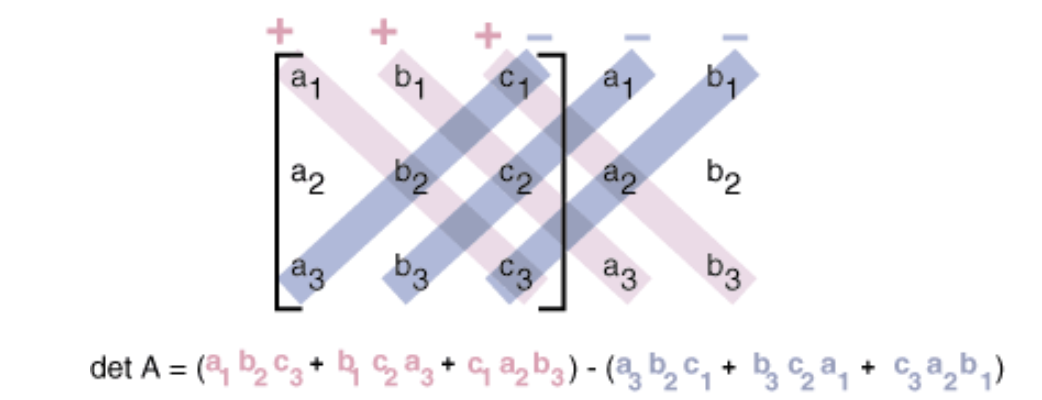
\includegraphics[width=1\textwidth]{images/3x3det.png}
    \end{center}

    \begin{Example}
        Let
        $$
        A=\left(\begin{array}{rrr}
        1 & 3 & -3 \\
        -3 & -5 & 2 \\
        -4 & 4 & -6
        \end{array}\right) \in \mathrm{M}_{3 \times 3}(R) .
        $$

        Using cofactor expansion along the first row of $A$, we obtain
        $$
        \begin{aligned}
        \operatorname{det}(A)= & (-1)^{1+1} A_{11} \cdot \operatorname{det}\left(\tilde{A}_{11}\right)+(-1)^{1+2} A_{12} \cdot \operatorname{det}\left(\tilde{A}_{12}\right) \\
        & +(-1)^{1+3} A_{13} \cdot \operatorname{det}\left(\tilde{A}_{13}\right) \\
        = & (-1)^2(1) \cdot \operatorname{det}\left(\begin{array}{rr}
        -5 & 2 \\
        4 & -6
        \end{array}\right)+(-1)^3(3) \cdot \operatorname{det}\left(\begin{array}{rr}
        -3 & 2 \\
        -4 & -6
        \end{array}\right) \\
        & \quad+(-1)^4(-3) \cdot \operatorname{det}\left(\begin{array}{rr}
        -3 & -5 \\
        -4 & 4
        \end{array}\right) \\
        = & 1[-5(-6)-2(4)]-3[-3(-6)-2(-4)]-3[-3(4)-(-5)(-4)] \\
        = & 1(22)-3(26)-3(-32) \\
        = & 40 .
        \end{aligned}
        $$
    \end{Example}

    \subsubsection*{Properties of determinants}

    \begin{enumerate}
        \item If $B$ is a matrix obtained by interchanging any two rows or interchanging any two columns of an $n \times n$ matrix $A$, then $\operatorname{det}(B)=-\operatorname{det}(A)$.

        \item If $B$ is a matrix obtained by multiplying each entry of some row or column of an $n \times n$ matrix $A$ by a scalar $k$, then $\operatorname{det}(B)=k \cdot \operatorname{det}(A)$.

        \item If $B$ is a matrix obtained from an $n \times n$ matrix $A$ by adding a multiple of row $i$ to row $j$ or a multiple of column $i$ to column $j$ for $i \neq j$, then $\operatorname{det}(B)=\operatorname{det}(A)$.

        As an example of the use of these three properties in evaluating determinants, let us compute the determinant of the $4 \times 4$ matrix $A$ considered previously. Our procedure is to introduce zeros into the second column of $A$ by employing property 3, and then to expand along that column. (The elementary row operations used here consist of adding multiples of row 1 to rows 2 and 4.) This procedure yields
        $$
        \begin{aligned}
        \operatorname{det}(A) & =\operatorname{det}\left(\begin{array}{rrrr}
        2 & 1 & 1 & 5 \\
        1 & 1 & -4 & -1 \\
        2 & 0 & -3 & 1 \\
        3 & 6 & 1 & 2
        \end{array}\right)=\operatorname{det}\left(\begin{array}{rrrr}
        2 & 1 & 1 & 5 \\
        -1 & 0 & -5 & -6 \\
        2 & 0 & -3 & 1 \\
        -9 & 0 & -5 & -28
        \end{array}\right) \\
        & =1(-1)^{1+2} \operatorname{det}\left(\begin{array}{rrr}
        -1 & -5 & -6 \\
        2 & -3 & 1 \\
        -9 & -5 & -28
        \end{array}\right) .
        \end{aligned}
        $$

        The resulting determinant of a $3 \times 3$ matrix can be evaluated in the same manner: Use type 3 elementary row operations to introduce two zeros into the first column, and then expand along that column. This results in the value $-102$. Therefore
        $$
        \operatorname{det}(A)=1(-1)^{1+2}(-102)=102
        $$

        \item The determinant of an upper triangular matrix is the product of its diagonal entries. In particular, $\operatorname{det}(I)=1$.

        \item If two rows (or columns) of a matrix are identical, then the determinant of the matrix is zero.

        As an illustration of property 4, notice that
        $$
        \operatorname{det}\left(\begin{array}{rrr}
        -3 & 1 & 2 \\
        0 & 4 & 5 \\
        0 & 0 & -6
        \end{array}\right)=(-3)(4)(-6)=72.
        $$

        \item For any $n \times n$ matrices $A$ and $B$, $\operatorname{det}(A B)=\operatorname{det}(A) \cdot \operatorname{det}(B)$.

        \item An $n \times n$ matrix $A$ is invertible if and only if $\operatorname{det}(A) \neq 0$. Furthermore, if $A$ is invertible, then $\operatorname{det}\left(A^{-1}\right)=\frac{1}{\operatorname{det}(A)}$.

        \item For any $n \times n$ matrix $A$, the determinants of $A$ and $A^{t}$ are equal.

        For example, property 7 guarantees that the matrix $A$ on page 233 is invertible because $\operatorname{det}(A)=102$.

        The final property, stated as Exercise 15 of Section 4.3, is used in Chapter 5. It is a simple consequence of properties 6 and 7.

        \item If $A$ and $B$ are similar matrices, then $\operatorname{det}(A)=\operatorname{det}(B)$.
    \end{enumerate}


    \section{Roots of a polynomial}
    The process of finding the roots of a polynomial can be either very straight forward or very complicated. Over the time we've developed multiple tools that help us in this task, we'll list a few of them to help us work with the characteristic polynomial. The most useful method for finding roots is to factorize the polynomials into factors of the form $(x - c)$ where $c$ is a real number, or find quadratic factors to then apply the quadratic formula. To find these factors we can use the synthetic division algorithm.

    \begin{thBox}
        \textit{\textbf{Fundamental Theorem Of Algebra}}. Every polynomial with complex coefficients has at least one complex zero.
    \end{thBox}

    \begin{thBox}
        \textit{\textbf{Roots theorem}}. Every polynomial of degree $n \geq 1$ has exactly $n$ zeros, provided that a zero of multiplicity $k$ is counted $k$ times.
    \end{thBox}

    \begin{thBox}
        \textit{\textbf{Rational Zeros Theorem}}. If the polynomial $P(x)=a_n x^n+a_{n-1} x^{n-1}+\cdots+a_1 x+a_0$ has integer coefficients, then every rational zero of $P$ is of the form
        $$
        \frac{p}{q}
        $$
        where $\quad p$ is a factor of the constant coefficient $a_0$
        and $\quad q$ is a factor of the leading coefficient $a_n$.
    \end{thBox}

    \begin{noteBox}
        \textit{\textbf{Finding the Rational Zeros of a Polynomial}}.
        \begin{enumerate}
            \item List Possible Zeros. List all possible rational zeros using the Rational Zeros Theorem.
            \item Divide. Use synthetic division to evaluate the polynomial at each of the candidates for rational zeros that you found in Step 1. When the remainder is 0 , note the quotient you have obtained.
            \item Repeat. Repeat Steps 1 and 2 for the quotient. Stop when you reach a quotient that is quadratic or factors easily, and use the quadratic formula or factor to find the remaining zeros.
        \end{enumerate}
    \end{noteBox}

    \chapter{Eigenvalues and Eigenvectors}

    \begin{defBox}
        \textit{\textbf{Eigenvector and Eigenvalues}}. Definitions. Let $\mathrm{T}$ be a linear operator on a vector space V. A nonzero vector $v \in \mathrm{V}$ is called an eigenvector of $\mathrm{T}$ if there exists a scalar $\lambda$ such that $\mathrm{T}(v)=\lambda v$. The scalar $\lambda$ is called the eigenvalue corresponding to the eigenvector $v$.\\

        Let $A$ be in $\mathrm{M}_{n \times n}(F)$. A nonzero vector $v \in \mathrm{F}^n$ is called an eigenvector of $A$ if $v$ is an eigenvector of $\mathrm{L}_A$; that is, if $A v=\lambda v$ for some scalar $\lambda$. The scalar $\lambda$ is called the eigenvalue of $A$ corresponding to the eigenvector $v$.
    \end{defBox}

    \begin{thBox}
        Let $T$ be a linear operator over a finite dimensional vector space $V$. And let $\lambda$ be a scalar, then the following are equivalent

        \begin{enumerate}
            \item $\lambda$ is an eigenvalue of $T$
            \item The operator $(T - \lambda I)$ is singular (it doesn't have inverse)
            \item $\det(T-\lambda I) = 0$
        \end{enumerate}
    \end{thBox}

    \begin{defBox}
        If $A$ is a matrix over a field $F$, an eigenvalue of $A$ in $F$ is a scalar in $F$, such that $(A - \lambda I)$ is singular.
    \end{defBox}

    \begin{defBox}
        Let $A$ be an squared matrix. The function $P_A: \mathbb{R} \to \mathbb{R}$ where $P_A(\lambda) = \det(A - \lambda I)$ is called the characteristic polynomial of $A$.
    \end{defBox}

    With these theorems and definitions, we can obtain eigenvalues of a matrix by finding the roots of the characteristic polynomial and obtain the eigenvector $v$ corresponding to an eigenvalue $\lambda$ by solving the system $(A-\lambda I)v = 0$

    \begin{Example}
        Let
        $$A = \begin{bmatrix}
            -1 & -3 & 9\\
            0 & 5 & 18\\
            0 & -2 & -7
        \end{bmatrix}$$
        To find the eigenvalues, eigenvectors, and the characteristic polynomial, we start with

        $$f(\lambda) = \det\left(A - \lambda I\right)$$

        Then, \begin{align*}
            \det\left(A - \lambda I\right) &= \det\left(
                \begin{bmatrix}
                    -1 & -3 & 9\\
                    0 & 5 & 18\\
                    0 & -2 & -7
                \end{bmatrix}
            - \lambda
                \begin{bmatrix}
                    1 & 0 & 0\\
                    0 & 1 & 0\\
                    0 & 0 & 1
                \end{bmatrix}
            \right)\\\\
            &= \det\left(
                \begin{bmatrix}
                    -1-\lambda & -3 & 9\\
                    0 & 5-\lambda & 18\\
                    0 & -2 & -7-\lambda
                \end{bmatrix}
            \right)\\\\
            &= -\lambda^3 -3\lambda^2 -3\lambda -1
        \end{align*}

        Now, to find the eigenvalues, we need to find the roots of the polynomial. It can be observed that $-\lambda^3 -3\lambda^2 -3\lambda -1$ is in the expanded form of a cube of a binomial, therefore, the polynomial can be factorized as follows:

        $$-(\lambda + 1)^3$$

        Thus, by setting $-(\lambda + 1)^3 = 0$, we can conclude that $\lambda_1 = -1, \lambda_2 = -1, \lambda_3 = -1$. Now let's find the eigenvectors, for this, we will solve the following homogeneous system: $Ax = 0$, where $x = (x_1, x_2, x_3)$ and $x_1, x_2, x_3 \in F$. So, the homogeneous system for $\lambda = -1$ would be as follows:
        \begin{align*}
            \begin{bmatrix}
                0 & -3 & 9\\
                0 & 6 & 18\\
                0 & -2 & -6
            \end{bmatrix}
            \begin{bmatrix}
                x_1\\ x_2\\ x_3
            \end{bmatrix} = \begin{bmatrix}
                0\\0\\0
            \end{bmatrix}
        \end{align*}

        Solving the system, we find that the vector

        $$\begin{bmatrix}
            1\\0\\0
        \end{bmatrix}$$

        is a solution to the system and therefore is an eigenvector for $A$.
    \end{Example}

    \begin{defBox}
        Let $\mathrm{T}$ be a linear operator on a vector space $\mathrm{V}$, and let $\lambda$ be an eigenvalue of $\mathrm{T}$. Define $\mathrm{E}_\lambda=\{x \in \mathrm{V}: \mathrm{T}(x)=\lambda x\}=\mathrm{N}\left(\mathrm{T}-\lambda \mathrm{I}_{\mathrm{V}}\right)$. The set $\mathrm{E}_\lambda$ is called the eigenspace of $\mathrm{T}$ corresponding to the eigenvalue $\lambda$. Analogously, we define the eigenspace of a square matrix $A$ corresponding to the eigenvalue $\lambda$ to be the eigenspace of $\mathrm{L}_A$ corresponding to $\lambda$.
    \end{defBox}

    Continuing with the previous example, its eigenspace $E_\lambda$ would be

    $$ E_\lambda = \left\{ \begin{bmatrix}1\\0\\0\end{bmatrix} \right\}$$

    \section{Working with the characteristic polynomial}
    It's worth to remember some tools to find the determinants of a matrix and the roots of a polynomial. Let's first remember the definition of determinant.

    We'll first state a theorem that will help us to find some parts of the characteristic polynomial.

    \begin{thBox}
        Denote the $n$ eigenvalues of a $A \in M_n(c)$, by $\lambda_1, \lambda_2, \dots , \lambda_n$ and its characteristic polynomial by

        $$P_a(\lambda) = (-1)^n\lambda^n + C_{n-1}\lambda^{n-1} + \cdots + C_1\lambda + C_0$$

        Then $$C_0 = \det(A) = \lambda_1 \lambda_2 \cdots \lambda_n$$ and $$(-1)^{n-1}C_{n-1} = tr(A) = \lambda_1 + \lambda_2 + \cdots + \lambda_n$$
    \end{thBox}

    \chapter{Diagonalization of a Matrix}

    \section{Multiplicity}

    \begin{defBox}
        \textit{\textbf{Geometrical multiplicity of an eigenvalue}}. Let $A$ be a squared matrix with the eigenvalue $\lambda$. The geometrical multiplicity of $\lambda$ is the dimension of $E_\lambda$ (The space generated by $\lambda$).
    \end{defBox}

    For example 1.2.5, the geometrical multiplicity of $\lambda = -1$ is $1$ since
    $$E_\lambda = \left\{ \begin{bmatrix}1\\0\\0\end{bmatrix} \right\}$$

    \begin{defBox}
        Let $A$ be a squared matrix with the eigenvalue $\lambda$. The algebraic multiplicity of $\lambda$ is the largest positive integer $k$ for which $(t-\lambda)^k$ is a factor of $f(t)$.
    \end{defBox}

    \begin{Example}
        Let

        $$A =\begin{pmatrix}
            3 & 1 & 0\\
            0 & 3 & 4\\
            0 & 0 & 4
        \end{pmatrix}$$

        which has characteristic polynomial $f(t) = -(t-3)^2(t-4)$. Hence $\lambda = 3$ is an eigenvalue of $A$ with multiplicity of 2, and $\lambda = 4$ is an eigenvalue of $A$ with multiplicity 1.
    \end{Example}

    \begin{thBox}
        Let $T$ be a linear operation on a finite-dimensional vector space $V$. And let $\lambda$ be an eigenvalue of $T$. Having algebraic multiplicity of $m$. Then $1 \leq dim(E_\lambda) \leq m$.
    \end{thBox}

    \section{Similar matrices}

    \begin{defBox}
        \textit{\textbf{Similar matrices}}. Two square matrices $A$ and $B$ are said to be similar if there exists a non-singular matrix $P$ such that

        $$B = P^{-1}AP$$
    \end{defBox}

    \begin{thBox}
        Let $A \in \mathrm{M}_{n \times n}(F)$, and let $\gamma$ be an ordered basis for $\mathrm{F}^n$. Then $\left[\mathrm{L}_A\right]_\gamma=Q^{-1} A Q$, where $Q$ is the $n \times n$ matrix whose $j$ th column is the $j$ th vector of $\gamma$.
    \end{thBox}

    \begin{thBox}
        Similar matrices have the same eigenvalues counting multiplicity.
    \end{thBox}

    \section{Diagonalization of a Matrix}


    \begin{defBox}
        Let $\mathcal{T}$ be the set of all linear transformations from $V$ into $W$, and let $L(V,W) = \{T \mid T \in \mathcal{T}\}$, then $L(V,W)$ is a vector space where its operations are defined as:

        \begin{itemize}
            \item \textit{\textbf{Vector addition}}. Let $T_1, T_2 \in L(V,W)$ then for every $v_1 \in V$
            $$(T_1+T_2)(v_1) = T_1(v_1) + T_2(v_1)$$
            \item \textit{\textbf{Scalar multiplication}}. Let $T \in L(V,W)$ and let $\alpha \in F$, then for all $v_1 \in V$
            $$(\alpha T)(v_1) = \alpha T(v_1)$$
        \end{itemize}
    \end{defBox}

    \begin{defBox}
        \textit{\textbf{Matrix left multiplication}}. Let $A$ be an $m \times n$ matrix with entries from a field $F$. We denote by $\mathrm{L}_A$ the mapping $\mathrm{L}_A: \mathrm{F}^n \rightarrow \mathrm{F}^m$ defined by $\mathrm{L}_A(x)=A x$ (the matrix product of $A$ and $x$ ) for each column vector $x \in \mathrm{F}^n$. We call $\mathrm{L}_A$ a left-multiplication transformation.
    \end{defBox}

    \begin{defBox}
        \textit{\textbf{Diagonal matrix}}. A matrix is called diagonal if all its entries $A_{ij}$ are zero except when $i = j$.
    \end{defBox}

    \begin{defBox}
        \textit{\textbf{Diagonalization of a Matrix}}. A linear operator $\mathrm{T}$ on a finite-dimensional vector space $\mathrm{V}$ is called diagonalizable if there is an ordered basis $\beta$ for $\mathrm{V}$ such that $[\mathrm{T}]_\beta$ is a diagonal matrix.

        A square matrix $A$ is called diagonalizable if $\mathrm{L}_A$ is diagonalizable. In other words we say that an squared matrix $A$ is diagonalizable if and only if there exists an invertible matrix $P$ such that

        $$D = P^{-1}AP$$ or
        $$A = PDP^{-1}$$
    \end{defBox}

    \begin{thBox}
        If $A$ is similar to a diagonal matrix $D$, then the elements of $D$ are the eigenvalues of $A$; And the values are independent of the form in which a linear transformation is represented.
    \end{thBox}

    \begin{thBox}
        A $nxn$ matrix is diagonalizable if and only if admits a linearly independent eigenvectors.
    \end{thBox}

    \begin{thBox}
        The following are equivalent

        \begin{enumerate}
            \item $T: V \to V$ is diagonalizable
            \item For every eigenvalue $\lambda$ of $T$, the geometric multiplicity of $\lambda$ coincides with the algebra multiplicity.
        \end{enumerate}
    \end{thBox}

    \section{Change of Basis}

    \begin{defBox}
        \textit{\textbf{Ordered basis}}. Let $V$ be a finite-dimensional vector space. An ordered basis for such space is endowed with a specific order, that is, an ordered basis for $V$ is a sequence of linearly independent vectors in $V$ that generate $V$.
    \end{defBox}

    \begin{Example}
        Let $V = F^3$.

        $$\beta = \left\{ e_1, e_2, e_3 \right\}$$
        $$\alpha = \left\{ e_2, e_1, e_3 \right\}$$

        Then $\beta \not = \alpha$. And $\beta, \alpha$ are ordered basis.
    \end{Example}

    \begin{defBox}
        Let $\beta = \left\{ u_1, u_2, \dots , u_n \right\}$ be an ordered basis for $V$. For each $v \in V$, let $\alpha_1, \alpha_2, \dots , \alpha_n$ be the unique scalars such that

        $$v = \sum_{i=1}^{n}\alpha_iu_i$$

        We define the coordinate vector of $v$ relative to $\beta$, denoted by

        $$[v]_\beta = \begin{pmatrix}
            \alpha_1\\ \alpha_2 \\ \vdots \\ \alpha_n
        \end{pmatrix}$$
    \end{defBox}

    \begin{Example}
        Let $P_2(\mathbb{R})$ and let $\beta = \left\{ 1, x, x^2 \right\}$ and $\alpha = \left\{ x^2, x, 1 \right\}$ if $v = f(x) = 4 + 6x -7x^2$.

        $$[v]_\beta = \begin{pmatrix}
            4\\6\\-7
        \end{pmatrix}$$

        $$[v]_\alpha = \begin{pmatrix}
            -7\\6\\4
        \end{pmatrix}$$
    \end{Example}

    \begin{thBox}
        Let $\beta = \left\{ u_1, u_2, \dots , u_n \right\}$ an ordered basis for $V$, then a coordinate map

        $$[]_\beta: V \to \mathbb{R}^n$$
        $$V \to [v]_\beta$$

        Is a linear transformation from $V \to \mathbb{R}^n$
    \end{thBox}

    \begin{defBox}
        We call $mxn$ matrix $A$ defined by $A_{ij} = a_{ij}$. The matrix representation of $T$ in the ordered basis $\beta$ and $\beta'$ and write $A = [T]_\beta$.\\

        If $V = W$ and $\beta = \beta'$, then $A = [T]_\beta$.
    \end{defBox}

    \begin{Example}
        Let $\beta = \{u_1, u_2, \dots , u_n\}$ be an ordered basis for $V$, and let $T$ be a coordinate mapping such that $T(v) = [v]_\beta$. Then $T$ is a linear transformation.

        \textit{\textbf{Proof}}. First, let's show that $T(v + w) = T(v) + T(w)$ for all $v, w \in V$.

        Let $v, w \in V$. We have:

        $$T(v) = [v]_\beta = \begin{bmatrix}
            \alpha_1\\ \alpha_2\\ \vdots \\ \alpha_n
        \end{bmatrix}$$

        where $\alpha_1,\dots, \alpha_n$ are scalars such that

        $$v = \sum_{i=1}^{n} \alpha_i u_i$$

        and similarly,

        $$T(w) = [w]_\beta = \begin{bmatrix}
            \gamma_1\\ \gamma_2\\ \vdots \\ \gamma_n
        \end{bmatrix}$$

        where $\gamma_1,\dots, \gamma_n$ are scalars such that

        $$w = \sum_{i=1}^{n} \gamma_i u_i$$

        Therefore,

        \begin{align*}
        T(v + w) &= [v + w]_\beta \\
        &= \left[\sum_{i=1}^{n} (\alpha_i + \gamma_i) u_i\right]_\beta \\
        &= \begin{bmatrix}
            \alpha_1 + \gamma_1\\ \alpha_2 + \gamma_2\\ \vdots \\ \alpha_n + \gamma_n
        \end{bmatrix} \\
        &= \begin{bmatrix}
            \alpha_1\\ \alpha_2\\ \vdots \\ \alpha_n
        \end{bmatrix} + \begin{bmatrix}
            \gamma_1\\ \gamma_2\\ \vdots \\ \gamma_n
        \end{bmatrix} \\
        &= T(v) + T(w)
        \end{align*}

        Next, let's show that $T(cv) = cT(v)$ for all $c \in \mathbb{R}$ and all $v \in V$.

        Let $v \in V$ and $c \in \mathbb{R}$. Then we have:

        $$T(v) = [v]_\beta = \begin{bmatrix}
            \alpha_1\\ \alpha_2\\ \vdots \\ \alpha_n
        \end{bmatrix}$$

        where $\alpha_1,\dots, \alpha_n$ are scalars such that

        $$v = \sum_{i=1}^{n} \alpha_i u_i$$

        So,

        \begin{align*}
        T(cv) &= [cv]_\beta \\
        &= \left[\sum_{i=1}^{n} (c\alpha_i) u_i\right]_\beta \\
        &= \begin{bmatrix}
            c\alpha_1\\ c\alpha_2\\ \vdots \\ c\alpha_n
        \end{bmatrix} \\
        &= c\begin{bmatrix}
            \alpha_1\\ \alpha_2\\ \vdots \\ \alpha_n
        \end{bmatrix} \\
        &= cT(v)
        \end{align*}

        Thus, $T$ is a linear transformation.

    \end{Example}

    \begin{Example}
        Sea $T: \mathcal{M}_{2x2}(\mathbb{R}) \to P_2(\mathbb{R})$ tal que

        $$T\left(\begin{bmatrix}
            a & b \\
            c & d
        \end{bmatrix}\right)$$

        y sean $\beta_1$ y $\beta_2$ bases de $\mathcal{M}_{2x2}(\mathbb{R})$ y $P_2(\mathbb{R})$ tal que

        $$\beta_1 = \left\{
            \begin{bmatrix}
                1 & 0 \\
                0 & 0
            \end{bmatrix},
            \begin{bmatrix}
                0 & 1 \\
                0 & 0
            \end{bmatrix},
            \begin{bmatrix}
                0 & 0 \\
                1 & 0
            \end{bmatrix},
            \begin{bmatrix}
                0 & 0 \\
                0 & 1
            \end{bmatrix}
        \right\}$$

        $$\beta_2 = \left\{1, x, x^2\right\}$$

        Encuentre $[T]_{\beta_1}^{\beta_2}$.

        Para encontrar $[T]_{\beta_1}^{\beta_2}$ debemos aplicar la transformación a cada vector de $\beta_1$ y luego obtener la matriz de la transformación. En este orden de ideas, para $v_j \in \beta_1$ tenemos lo siguiente:

        $$T(v_1) = T \left(\begin{bmatrix}
            1 & 0 \\
            0 & 0
        \end{bmatrix}\right) = (1 + 0) + 2\cdot 0x + 0x^2 = 1$$

        $$T(v_2) = T \left(\begin{bmatrix}
            0 & 1 \\
            0 & 0
        \end{bmatrix}\right) = (0 + 1) + 2\cdot 0x + 1x^2 = 1 + x^2$$

        $$T(v_3) = T \left(\begin{bmatrix}
            0 & 0 \\
            1 & 0
        \end{bmatrix}\right) = (0 + 0) + 2\cdot 0x + 0x^2 = 0$$

        $$T(v_4) = T \left(\begin{bmatrix}
            0 & 0 \\
            0 & 1
        \end{bmatrix}\right) = (0 + 0) + 2\cdot 1x + 0x^2 = 2x$$

        Luego

        $$[T]_{\beta_1}^{\beta_2} = \begin{bmatrix}
            1 & 1 & 0 & 0\\
            0 & 0 & 0 & 2\\
            0 & 1 & 0 & 0
        \end{bmatrix}$$
    \end{Example}

    \begin{Example}
            Let $T: \mathcal{M}_{2 \times 2}(\mathbb{R}) \to P_2(\mathbb{R})$ be such that

        $$T\left(\begin{bmatrix}
            a & b \\
            c & d
        \end{bmatrix}\right)$$

        and let $\beta_1$ and $\beta_2$ be bases of $\mathcal{M}_{2 \times 2}(\mathbb{R})$ and $P_2(\mathbb{R})$ respectively, given by

        $$\beta_1 = \left\{
            \begin{bmatrix}
                1 & 0 \\
                0 & 0
            \end{bmatrix},
            \begin{bmatrix}
                0 & 1 \\
                0 & 0
            \end{bmatrix},
            \begin{bmatrix}
                0 & 0 \\
                1 & 0
            \end{bmatrix},
            \begin{bmatrix}
                0 & 0 \\
                0 & 1
            \end{bmatrix}
        \right\}$$

        $$\beta_2 = \left\{1, x, x^2\right\}$$

        Find $[T]_{\beta_1}^{\beta_2}$.

        To find $[T]_{\beta_1}^{\beta_2}$, we must apply the transformation to each vector in $\beta_1$ and then obtain the matrix of the transformation. In this vein, for $v_j \in \beta_1$ we have the following:

        $$T(v_1) = T \left(\begin{bmatrix}
            1 & 0 \\
            0 & 0
        \end{bmatrix}\right) = (1 + 0) + 2 \cdot 0x + 0x^2 = 1$$

        $$T(v_2) = T \left(\begin{bmatrix}
            0 & 1 \\
            0 & 0
        \end{bmatrix}\right) = (0 + 1) + 2 \cdot 0x + 1x^2 = 1 + x^2$$

        $$T(v_3) = T \left(\begin{bmatrix}
            0 & 0 \\
            1 & 0
        \end{bmatrix}\right) = (0 + 0) + 2 \cdot 0x + 0x^2 = 0$$

        $$T(v_4) = T \left(\begin{bmatrix}
            0 & 0 \\
            0 & 1
        \end{bmatrix}\right) = (0 + 0) + 2 \cdot 1x + 0x^2 = 2x$$

        Then

        $$[T]_{\beta_1}^{\beta_2} = \begin{bmatrix}
            1 & 1 & 0 & 0 \\
            0 & 0 & 0 & 2 \\
            0 & 1 & 0 & 0
        \end{bmatrix}$$

        Let $F: \mathbb{R}^3 \to \mathbb{R}^2$ be defined as

        $$F(x, y, z) = (3x + 2y - 4z, x - 5y + 3z)$$

        \begin{enumerate}
            \item Find the matrix of $F$ for the following bases of $\mathbb{R}^3$ and $\mathbb{R}^2$

            $$\beta_1 = \{(1,1,1), (1,1,0), (1,0,0)\}$$
            $$\beta_2 = \{(1,3), (2,5)\}$$

            \item Given $V \in \mathbb{R}^3$, verify
            $$[F]_{\beta_1}^{\beta_2}[v]_{\beta_1} = [F(v)]_{\beta_2}$$
        \end{enumerate}

        \begin{enumerate}
            \item By definition of $F$,
            $$F((1,1,1)) = (3(1) + 2(1) - 4(1), 1 - 5(1) + 3(1)) = (1, -1)$$
            $$F((1,1,0)) = (3(1) + 2(1) - 4(0), 1 - 5(1) + 3(0)) = (5, -4)$$
            and
            $$F((1,0,0)) = (3(1) + 2(0) - 4(0), 1 - 5(0) + 3(0)) = (3, 1)$$

            Then
            $$\begin{bmatrix}
                1 \\ -1
            \end{bmatrix}_{\beta_2} = \begin{bmatrix}
                -7 \\ 1
            \end{bmatrix}$$
            $$\begin{bmatrix}
                5 \\ -4
            \end{bmatrix}_{\beta_2} = \begin{bmatrix}
                -33 \\ 19
            \end{bmatrix}$$
            $$\begin{bmatrix}
                3 \\ -1
            \end{bmatrix}_{\beta_2} = \begin{bmatrix}
                -13 \\ 8
            \end{bmatrix}$$

            Finally,

            $$[F]_{\beta_1}^{\beta_2} = \begin{bmatrix}
                -7 & -33 & -13 \\
                1 & 19 & 8
            \end{bmatrix}$$

            \item Let $v = (a, b, c)$. We have

            $$[F(v)]_{\beta_2} = \begin{bmatrix}
                a \\ b
            \end{bmatrix}_{\beta_2} = \begin{bmatrix}
                \begin{bmatrix}
                    1 & 2 & 3a + 2b - 4c \\
                    3 & 5 & a - 5b + 3c
                \end{bmatrix} = \begin{bmatrix}
                    -13a - 20b + 26c \\
                    8a + 11b - 15c
                \end{bmatrix}
            \end{bmatrix}$$

            Similarly, we have

            $$[v]_{\beta_1} = \begin{bmatrix}
                c \\ b - c \\ a - b
            \end{bmatrix}$$

            Finally

            \begin{align*}
                [F]_{\beta_1}^{\beta_2}[v]_{\beta_1} &=
                \begin{bmatrix}
                    -7 & -33 & -13 \\
                    1 & 19 & 8
                \end{bmatrix} \begin{bmatrix}
                    c \\
                    b - c \\
                    a - b
                \end{bmatrix} \\
                &= \begin{bmatrix}
                    -13a - 20b + 26c \\
                    8a + 11b - 15c
                \end{bmatrix} \\
                &= [F(v)]_{\beta_2}
            \end{align*}
        \end{enumerate}
    \end{Example}

    \begin{thBox}
        If $T: V \to V$ is a linear operator and $\beta = \left\{ \alpha_1, \dots , \alpha_n \right\}$ and $\beta' = \left\{ \alpha_1', \dots , \alpha_n' \right\}$ two ordered bases for $V$, there exists a matrix $P \in M_{nxn}$ invertible such that

        $$[T]_{\beta'} = P^{-1}[T]P$$
    \end{thBox}

    \begin{thBox}
        Let $V$ and $W$ be finite dimensional vector space $V$ with the ordered bases $\beta$ and $\gamma$, respectively and let $T: V \to W$ be a linear transformation, for every $v \in V$, we have

        $$[T(v)]_\gamma = [T]_\beta^\gamma[v]_\beta$$
    \end{thBox}

    \begin{thBox}
        If $T: V \to W$ is a linar transformation, such that $T \in L(V, W)$, and $\beta = \left\{ \alpha_1, \dots \alpha_n \right\}$ a base for $V$, and $\beta' = \left\{ \alpha_1', \dots \alpha_n' \right\}$ be a base for $W$, then there exists a unique matrix $A \in M_{nxn}$ such that for each $x \in V$

        $$[T(x)]_\beta = A[x]_\beta$$
    \end{thBox}

    \section{Sum of subspaces}

    \begin{defBox}
        \textit{\textbf{Sum of sets}}. Suppose that $U_1, \dots U_m$ are subsets of a vector space $V$. Then the sum of $U_1, \dots , U_m$ denoted by $U_1 + \cdots + U_m $ is the set of all possible sums of the elements of $U_1, \dots , U_m$, more precisely

        $$U_1 + \cdots U_m = \left\{ u_1 + \cdots u_m \mid u_1 \in U_1 , \dots , u_m \in U_m \right\}$$
    \end{defBox}

    \begin{Example}
        $$U = \left\{ (x, 0, 0) \in F^3 \mid x \in F \right\}$$
        $$W = \left\{ (0, y, 0) \in F^3 \mid x \in F \right\}$$

        Then

        $$U + W = \left\{ (x, y, 0) \in F^3 \mid x, y \in F \right\}$$
    \end{Example}

    \begin{Example}
        $$W_1 = \left\{ m(1,0) \mid m \in \mathbb{R} \right\}$$
        $$W_2 = \left\{ l(0,1) \mid l \in \mathbb{R} \right\}$$

        Then

        $$W_1 + W_2 = \left\{ m(1,0) + l(1,0) \mid m, l \in \mathbb{R} \right\}$$
    \end{Example}

    \begin{thBox}
        \textit{\textbf{The sum of subspaces is also a subspace}}. Let $V_1, \dots , V_n$ subspaces of a vector space $V$, then

        $$ V_1 + \cdots V_n $$
    \end{thBox}

    \chapter{Normed vector spaces}

    \section{Inner products}
    \begin{defBox}
        Let $\mathrm{V}$ be a vector space over a field $F$. An inner product on $\mathrm{V}$ is a function that assigns to every ordered pair of vectors $x$ and $y$ in $\mathrm{V}$ a scalar in $F$, denoted $\langle x, y\rangle$, such that for all $x, y, z$ in $\mathrm{V}$ and all $c$ in $F$, the following hold:

        (a) $\langle x+z, y\rangle=\langle x, y\rangle+\langle z, y\rangle$.

        (b) $\langle c x, y\rangle=c\langle x, y\rangle$.

        (c) $\overline{\langle x, y\rangle}=\langle y, x\rangle$, where the bar denotes complex conjugation.

        (d) If $x \neq 0$, then $\langle x, x\rangle$ is a positive real number.
    \end{defBox}

    This definition specifies the properties that an inner product must satisfy on a vector space, generalizing concepts like those of dot product in $\mathbb{R}^n$.


    \begin{Example}
        For $x=\left(a_{1}, a_{2}, \ldots, a_{n}\right)$ and $y=\left(b_{1}, b_{2}, \ldots, b_{n}\right)$ in $\mathrm{F}^{n}$, define

        $$
        \langle x, y\rangle=\sum_{i=1}^{n} a_{i} \bar{b}_{i}
        $$

        Thus, for $x=(1+i, 4)$ and $y=(2-3 i, 4+5 i)$ in $\mathrm{C}^{2}$,

        $$
        \langle x, y\rangle=(1+i)(2+3 i)+4(4-5 i)=15-15 i
        $$

        The inner product in this example is called the standard inner product on $\mathrm{F}^{n}$.
    \end{Example}

    This example shows how the standard inner product is calculated in $\mathrm{F}^{n}$, demonstrating that it satisfies the properties of an inner product.


    \begin{Example}
        If $\langle x, y\rangle$ is any inner product on a vector space $\mathrm{V}$ and $r>0$, define another inner product by $\langle x, y\rangle^{\prime}=r\langle x, y\rangle$. If $r \leq 0$, then condition (d) of the definition would not hold.
    \end{Example}

    Shows how scaling an inner product by a positive scalar results in another valid inner product.


    \begin{Example}
        Let $V=C([0,1])$, the vector space of real-valued continuous functions on $[0,1]$. For $f, g \in \mathrm{V}$, define $\langle f, g\rangle=\int_{0}^{1} f(t) g(t) d t$.
    \end{Example}

    Inner product defined in terms of an integral, demonstrating application in function spaces.


    \begin{defBox}
        Let $A \in \mathrm{M}_{m \times n}(F)$. We define the conjugate transpose or adjoint of $A$ to be the $n \times m$ matrix $A^{*}$ such that $\left(A^{*}\right)_{i j}=\bar{A}_{j i}$ for all $i, j$.
    \end{defBox}

    Defines the important concept of conjugate transpose, which is crucial in various linear algebra and functional analysis contexts.


    \begin{Example}
        Let

        \[
        A=\left(\begin{array}{ll}
        i & 1+2 i \\
        2 & 3+4 i
        \end{array}\right)
        \]

        Then

        \[
        A^{*}=\left(\begin{array}{cc}
        -i & 2 \\
        1-2 i & 3-4 i
        \end{array}\right)
        \]
    \end{Example}

    Provides a concrete example of calculating the conjugate transpose of a matrix with complex entries.


    \begin{Example}
        Let $\mathrm{V}=\mathrm{M}_{n \times n}(F)$, and define $\langle A, B\rangle=\operatorname{tr}\left(B^{*} A\right)$ for $A, B \in \mathrm{V}$.
    \end{Example}

    Defines an inner product on the vector space of matrices using the trace function, known as the Frobenius inner product.


    \begin{defBox}
        Let $\mathrm{V}$ be an inner product space. For $x \in \mathrm{V}$, we define the norm or length of $x$ by $\|x\|=\sqrt{\langle x, x\rangle}$.
    \end{defBox}

    Defines the norm of a vector in an inner product space, generalizing the concept of vector length.


    \begin{thBox}
        Theorem 6.2: Let $\mathrm{V}$ be an inner product space over $F$. Then for all $x, y \in \mathrm{V}$ and $c \in F$, the following statements are true.

        (a) $\|c x\|=|c| \cdot\|x\|$.

        (b) $\|x\|=0$ if and only if $x=0$. In any case, $\|x\| \geq 0$.

        (c) (Cauchy-Schwarz Inequality) $|\langle x, y\rangle| \leq\|x\| \cdot\|y\|$.

        (d) (Triangle Inequality) $\|x+y\| \leq\|x\|+\|y\|$.
    \end{thBox}

    This theorem establishes key properties and inequalities for norms and inner products, including the important Cauchy-Schwarz and Triangle inequalities.


    \begin{Example}
        For $\mathrm{F}^{n}$, we may apply (c) and (d) of Theorem 6.2 to the standard inner product to obtain well-known inequalities:

        \[
        \left|\sum_{i=1}^{n} a_{i} \bar{b}_{i}\right| \leq\left[\sum_{i=1}^{n}\left|a_{i}\right|^{2}\right]^{1 / 2}\left[\sum_{i=1}^{n}\left|b_{i}\right|^{2}\right]^{1 / 2}
        \]

        and

        \[
        \left[\sum_{i=1}^{n}\left|a_{i}+b_{i}\right|^{2}\right]^{1 / 2} \leq\left[\sum_{i=1}^{n}\left|a_{i}\right|^{2}\right]^{1 / 2}+\left[\sum_{i=1}^{n}\left|b_{i}\right|^{2}\right]^{1 / 2}
        \]
    \end{Example}

    Illustrates the application of Cauchy-Schwarz and Triangle inequalities in Euclidean space with standard inner products.


    \begin{defBox}
        Let $\mathrm{V}$ be an inner product space. Vectors $x$ and $y$ in $\mathrm{V}$ are orthogonal (or perpendicular) if $\langle x, y\rangle=0$. A subset $S$ of $\mathrm{V}$ is orthogonal if any two distinct vectors in $S$ are orthogonal. A vector $x$ in $\mathrm{V}$ is a unit vector if $\|x\|=1$. Finally, a subset $S$ of $\mathrm{V}$ is orthonormal if $S$ is orthogonal and consists entirely of unit vectors.
    \end{defBox}

    Defines concepts of orthogonality, unit vectors, and orthonormal sets in the context of inner product spaces.


    \begin{Example}
        In $\mathrm{F}^{3}, \{(1,1,0),(1,-1,1),(-1,1,2)\}$ is an orthogonal set of nonzero vectors, but it is not orthonormal. If we normalize the vectors, we get the orthonormal set:

        \[
        \left\{\frac{1}{\sqrt{2}}(1,1,0), \frac{1}{\sqrt{3}}(1,-1,1), \frac{1}{\sqrt{6}}(-1,1,2)\right\}
        \]
    \end{Example}

    Shows how to normalize a set of orthogonal vectors to form an orthonormal set.


    \begin{Example}
        Recall the inner product space $\mathrm{H}$. For any integer $n$, let $f_{n}(t)=e^{i n t}$, where $0 \leq t \leq 2 \pi$. Define $S=\left\{f_{n}: n \text { is an integer }\right\}$. Clearly $S$ is a subset of $\mathrm{H}$. For $m \neq n$,

        \[
        \left\langle f_{m}, f_{n}\right\rangle =\frac{1}{2 \pi} \int_{0}^{2 \pi} e^{i m t} \overline{e^{i n t}} d t=\frac{1}{2 \pi} \int_{0}^{2 \pi} e^{i(m-n) t} d t = 0
        \]
    \end{Example}

    Introduces an important orthonormal set in the context of continuous complex-valued functions on an interval, used in further examples and applications in analysis.

    \begin{defBox}
    A linear space over the field $\mathbf{F}$ of scalars is a set $V$ satisfying:
    \begin{enumerate}
        \item $V$ is closed under vector addition.
        \item Vector addition is commutative and associative.
        \item There is a zero element in $V$ such that $v + 0 = v$ for all $v$ in $V$.
        \item For each $v$ in $V$, there is an additive inverse $-v$ such that $v + (-v) = 0$.
        \item $V$ is closed under scalar multiplication.
        \item Scalar multiplication is associative and distributive.
        \item $1v = v$ for all $v$ in $V$.
    \end{enumerate}
    \end{defBox}

    \begin{Example}
    $\mathbf{R}^{n}$ with the usual operations is a vector space over $\mathbf{R}$.
    \end{Example}

    \begin{Example}
    $\mathbf{C}^{n}$ with the usual operations is a vector space over $\mathbf{C}$.
    \end{Example}

    \begin{Example}
    The set $C[a, b]$ of $\mathbf{F}$-valued continuous functions on $[a, b]$ is a linear space over $\mathbf{F}$.
    \end{Example}

    \begin{Example}
    The set $C^{k}[a, b]$ of $\mathbf{F}$-valued $k$-times continuously differentiable functions on $[a, b]$ is a linear space over $\mathbf{F}$.
    \end{Example}

    \begin{Example}
    The set $L^{1}(B)$ of functions $f: \mathbf{R}^{n} \rightarrow \mathbf{F}$ satisfying $\int_{B}|f(x)| dx < \infty$ is a linear space over $\mathbf{F}$.
    \end{Example}

    \begin{Example}
    The set $L^{2}(B)$ of functions $f: \mathbf{R}^{n} \rightarrow \mathbf{F}$ satisfying $\int_{B}|f(x)|^{2} dx < \infty$ is a linear space over $\mathbf{F}$.
    \end{Example}

    \begin{defBox}
    Let $V$ be a linear space. If $U \subseteq V$ is closed under vector addition and scalar multiplication, then $U$ is a subspace of $V$. A subspace is itself a linear space.
    \end{defBox}

    \begin{Example}
    Let $V=\mathbf{R}^{3}$. If $U$ is a subspace of $V$, then either
    \begin{enumerate}
        \item $U = \mathbf{R}^{3}$,
        \item $U$ is a plane through the origin,
        \item $U$ is a line through the origin,
        \item $U = \{0\}$.
    \end{enumerate}
    \end{Example}

    \begin{Example}
    Let $[a, b]$ be a finite interval. The set $C[a, b]$ is a subspace of $L^{1}[a, b]$.
    \end{Example}

    \begin{defBox}
    A norm $\| \cdot \|$ on a linear space $V$ is a mapping from $V$ to $\mathbf{R}$ satisfying:
    \begin{enumerate}
        \item $\|v \| \geq 0$ for all $v \in V$;
        \item $\|v \| = 0$ if and only if $v = 0$;
        \item $\|\alpha v\| = |\alpha| \|v \|$ for all $\alpha \in \mathbf{C}$ and $v \in V$;
        \item (Triangle inequality) $\| u + v \| \leq \| u \| + \| v \|$ for all $u, v \in V$.
    \end{enumerate}
    \end{defBox}

    \begin{Example}
    $\mathbf{F}^{n}$ is a normed linear space with $\| z \| = \{ |z_1|^2 + \cdots + |z_n|^2 \}^{1/2}$.
    \end{Example}

    \begin{Example}
    $C[a, b]$ is a normed linear space with the maximum (or $L^{\infty}$) norm $\| f \| = \max_{[a, b]} |f(x)|$.
    \end{Example}

    \begin{Example}
    $C^{k}[a, b]$ is a normed linear space with $\| f \| = \sum_{j=1}^{k} \max_{[a, b]} |f^{(j)}(x)|$.
    \end{Example}

    \begin{Example}
    $L^{1}(B)$ is a normed linear space with $\| f \| = \int_{B} |f(x)| dx$.
    \end{Example}

    \begin{Example}
    $L^{2}(B)$ is a normed linear space with $\| f \| = \{ \int_{B} |f(x)|^2 dx \}^{1/2}$.
    \end{Example}

    \begin{defBox}
    A sequence $\{v_k\}$ of vectors in a normed linear space $V$ is convergent if there is a $v \in V$ such that $\|v_k - v\| \rightarrow 0$ as $k \rightarrow \infty$.
    \end{defBox}

    \begin{defBox}
    A sequence $\{v_k\}$ of vectors in a normed linear space $V$ is Cauchy convergent if $\|v_m - v_n\| \rightarrow 0$ as $m, n \rightarrow \infty$.
    \end{defBox}

    \begin{defBox}
    A normed linear space is complete if all Cauchy convergent sequences are convergent. A complete normed linear space is called a Banach space.
    \end{defBox}

    \begin{Example}
    $C[a, b], C^{k}[a, b], L^{1}(B)$ and $L^{2}(B)$ are all Banach spaces with respect to the given norms.
    \end{Example}

    \begin{Example}
    Let $V$ be the set $C[0,2]$ of real-valued functions with norm $\|f \| = \int_{0}^{2} |f(x)| dx$. Although $V$ is a normed linear space, it is not a Banach space. The sequence $\{f_k\}$ with $f_k(x) = x^k$ for $0 \leq x < 1$ and $1$ for $1 \leq x \leq 2$ is Cauchy convergent in $V$ but does not converge to a function in $V$.
    \end{Example}

    \begin{defBox}
    An inner product on a linear space $V$ over $\mathbf{F}$ is a mapping $\langle \cdot, \cdot \rangle$ from $V \times V$ to $\mathbf{F}$ satisfying:
    \begin{enumerate}
        \item $\langle v, v \rangle \geq 0$ for all $v \in V$;
        \item $\langle v, v \rangle = 0$ if and only if $v = 0$;
        \item $\langle u, v \rangle = \langle v, u \rangle^{*}$ for all $u, v \in V$;
        \item $\langle \alpha u, v \rangle = \alpha \langle u, v \rangle$ for all $\alpha \in \mathbf{F}$ and $u, v \in V$;
        \item $\langle u+v, w \rangle = \langle u, w \rangle + \langle v, w \rangle$ for all $u, v, w \in V$.
    \end{enumerate}
    \end{defBox}

    \begin{Example}
    $\mathbf{F}^{n}$ is an inner product space: For $x = (x_1, \ldots, x_n)$ and $y = (y_1, \ldots, y_n)$ in $\mathbf{F}^{n}$, $\langle x, y \rangle = x_1 y_1^{*} + \cdots + x_n y_n^{*}$. When $\mathbf{F} = \mathbf{R}$, this reduces to the usual dot product on $\mathbf{R}^{n}$.
    \end{Example}

    \begin{Example}
    $L^{2}(B)$ is an inner product space with $\langle f, g \rangle = \int_{B} f(x) g(x)^{*} dx$.
    \end{Example}

    \begin{defBox}
    An inner product space that is complete with respect to the norm $\|v\| = \sqrt{\langle v, v \rangle}$ is called a Hilbert space.
    \end{defBox}

    \begin{Example}
    $\mathbf{C}^{n}$ and $L^{2}(B)$ are Hilbert spaces with the given inner products.
    \end{Example}

    \section{Orthagonalization}

    \begin{defBox}
        Let $\mathrm{V}$ be an inner product space. A subset of $\mathrm{V}$ is an orthonormal basis for $\mathrm{V}$ if it is an ordered basis that is orthonormal.
    \end{defBox}

    \begin{Example}
        The standard ordered basis for $\mathrm{F}^{n}$ is an orthonormal basis for $\mathrm{F}^{n}$.
    \end{Example}

    \begin{Example}
        The set
        $$
        \left\{\left(\frac{1}{\sqrt{5}}, \frac{2}{\sqrt{5}}\right),\left(\frac{2}{\sqrt{5}}, \frac{-1}{\sqrt{5}}\right)\right\}
        $$
        is an orthonormal basis for $\mathrm{R}^{2}$.
    \end{Example}

    \begin{thBox}
        \textbf{Theorem 6.3.} Let $\mathrm{V}$ be an inner product space and $S=\left\{v_{1}, v_{2}, \ldots, v_{k}\right\}$ be an orthogonal subset of $\mathrm{V}$ consisting of nonzero vectors. If $y \in \operatorname{span}(S)$, then
        $$
        y = \sum_{i=1}^{k} \frac{\left\langle y, v_{i}\right\rangle}{\left\|v_{i}\right\|^{2}} v_{i}
        $$
    \end{thBox}

    \begin{thBox}
        \textbf{Corollary 1.} If, in addition to the hypotheses of Theorem 6.3, $S$ is orthonormal and $y \in \operatorname{span}(S)$, then
        $$
        y = \sum_{i=1}^{k}\left\langle y, v_{i}\right\rangle v_{i}
        $$
    \end{thBox}

    \begin{thBox}
        \textbf{Corollary 2.} Let $\mathrm{V}$ be an inner product space, and let $S$ be an orthogonal subset of $\mathrm{V}$ consisting of nonzero vectors. Then $S$ is linearly independent.
    \end{thBox}

    \begin{Example}
        By Corollary 2, the orthonormal set
        $$
        \left\{\frac{1}{\sqrt{2}}(1,1,0), \frac{1}{\sqrt{3}}(1,-1,1), \frac{1}{\sqrt{6}}(-1,1,2)\right\}
        $$
        obtained in Example 8 of Section 6.1 is an orthonormal basis for $\mathrm{R}^{3}$. Let $x=(2,1,3)$. The coefficients given by Corollary 1 to Theorem 6.3 that express $x$ as a linear combination of the basis vectors are:
        $$
        a_{1}=\frac{1}{\sqrt{2}}(2+1)=\frac{3}{\sqrt{2}}, \quad a_{2}=\frac{1}{\sqrt{3}}(2-1+3)=\frac{4}{\sqrt{3}}
        $$
        and
        $$
        a_{3}=\frac{1}{\sqrt{6}}(-2+1+6)=\frac{5}{\sqrt{6}}
        $$
        Checking:
        $$
        (2,1,3)=\frac{3}{2}(1,1,0)+\frac{4}{3}(1,-1,1)+\frac{5}{6}(-1,1,2)
        $$
    \end{Example}

    \begin{thBox}
        \textbf{Theorem 6.4.} Let $\mathrm{V}$ be an inner product space and $S=\left\{w_{1}, w_{2}, \ldots, w_{n}\right\}$ be a linearly independent subset of $\mathrm{V}$. Define $S^{\prime}=\left\{v_{1}, v_{2}, \ldots, v_{n}\right\}$, where $v_{1}=w_{1}$ and
        $$
        v_{k}=w_{k}-\sum_{j=1}^{k-1} \frac{\left\langle w_{k}, v_{j}\right\rangle}{\left\|v_{j}\right\|^{2}} v_{j} \quad \text { for } 2 \leq k \leq n
        $$
        Then $S^{\prime}$ is an orthogonal set of nonzero vectors such that $\operatorname{span}\left(S^{\prime}\right)=\operatorname{span}(S)$.
    \end{thBox}

    \begin{Example}
        In $\mathrm{R}^{4}$, let $w_{1}=(1,0,1,0)$, $w_{2}=(1,1,1,1)$, and $w_{3}=(0,1,2,1)$. We use the Gram-Schmidt process to compute the orthogonal vectors $v_{1}$, $v_{2}$, and $v_{3}$.
        Take $v_{1}=w_{1}=(1,0,1,0)$. Then
        $$
        v_{2}=(0,1,0,1)
        $$
        and
        $$
        v_{3}=(-1,0,1,0)
        $$
        Normalizing, we get:
        $$
        u_{1}=\frac{1}{\sqrt{2}}(1,0,1,0), \quad u_{2}=\frac{1}{\sqrt{2}}(0,1,0,1), \quad u_{3}=\frac{1}{\sqrt{2}}(-1,0,1,0)
        $$
    \end{Example}

    \begin{Example}
        Let $\mathrm{V}=\mathrm{P}(R)$ with the inner product $\langle f(x), g(x)\rangle=\int_{-1}^{1} f(t) g(t) d t$. Consider $\mathrm{P}_{2}(R)$ with standard ordered basis $\beta$. We use Gram-Schmidt to obtain an orthonormal basis:
        $$
        \left\{1, x, x^{2}-\frac{1}{3}\right\} \rightarrow \left\{\frac{1}{\sqrt{2}}, \sqrt{\frac{3}{2}} x, \sqrt{\frac{5}{8}}(3 x^{2}-1)\right\}
        $$
    \end{Example}

    \begin{defBox}
        Let $\beta$ be an orthonormal subset of an inner product space $\mathrm{V}$, and let $x \in \mathrm{V}$. We define the Fourier coefficients of $x$ relative to $\beta$ to be the scalars $\langle x, y\rangle$, where $y \in \beta$.
    \end{defBox}

    \begin{Example}
        Compute the Fourier coefficients of $f(t)=t$ relative to $S=\left\{e^{int}: n \text{ is an integer}\right\}$.
        $$
        \left\langle f, f_{n}\right\rangle=\frac{-1}{i n} \text{ for } n \neq 0,
        $$
        $$
        \langle f, 1\rangle=\pi \text{ for } n=0
        $$
    \end{Example}

    \begin{defBox}
        Let $S$ be a nonempty subset of an inner product space V. We define $S^{\perp}$ (read "S perp") to be the set of all vectors in $\mathrm{V}$ that are orthogonal to every vector in $S$; that is, $S^{\perp}=\{x \in \mathrm{V}:\langle x, y\rangle=0$ for all $y \in S\}$. The set $S^{\perp}$ is called the orthogonal complement of $S$.
    \end{defBox}

    \begin{Example}
        Verify that $\{0\}^{\perp}=\mathrm{V}$ and $\mathrm{V}^{\perp}=\{0\}$ for any inner product space $\mathrm{V}$.
    \end{Example}

    \begin{Example}
        If $\mathrm{V}=\mathrm{R}^{3}$ and $S=\left\{e_{3}\right\}$, then $S^{\perp}$ equals the $xy$-plane.
    \end{Example}

    \begin{thBox}
        \textbf{Theorem 6.6.} Let $\mathrm{W}$ be a finite-dimensional subspace of an inner product space $\mathrm{V}$, and let $y \in \mathrm{V}$. Then there exist unique vectors $u \in \mathrm{W}$ and $z \in \mathrm{W}^{\perp}$ such that $y = u + z$. Furthermore, if $\left\{v_{1}, v_{2}, \ldots, v_{k}\right\}$ is an orthonormal basis for $\mathrm{W}$, then
        $$
        u = \sum_{i=1}^{k}\left\langle y, v_{i}\right\rangle v_{i}
        $$
    \end{thBox}

    \begin{Example}
        Let $\mathrm{V}=\mathrm{P}_{3}(R)$ with the inner product
        $$
        \langle f(x), g(x)\rangle=\int_{-1}^{1} f(t) g(t) d t \quad \text{for all } f(x), g(x) \in \mathrm{V}.
        $$
    \end{Example}


    \chapter{Dual spaces}
    \section{Notes}
    \begin{defBox}
        A linear functional on $V$ is a linear map $V \rightarrow \mathbb{F}$. In other words, a linear functional on $V$ is an element of $\mathcal{L}(V, \mathbb{F})$.
        \end{defBox}

        \begin{defBox}
        The dual space of $V$, denoted by $V^{*}$, is the space of all linear functionals on $V$; i.e. $V^{*} := \mathcal{L}(V, \mathbb{F})$.
        \end{defBox}

        \begin{defBox}
        Let $T: V \rightarrow W$ be linear. The dual map (or transpose) of $T$ is the map $T^{*}: W^{*} \rightarrow V^{*}$ defined by $T^{*} g = g T$ for all $g \in W^{*}$.
        \end{defBox}

        \begin{defBox}
        Let $U$ be a subspace of $V$. The annihilator of $U$ in $V^{*}$, denoted by $U^{\perp}$, is the set of linear functionals on $V$ which vanish on $U$; i.e. $U^{\perp} = \left\{ f \in V^{*} \mid f(u) = 0 \text{ for all } u \in U \right\}$.
        \end{defBox}

        \begin{thBox}
        Suppose that $V$ is finite-dimensional and let $\left(v_{1}, \ldots, v_{n}\right)$ be a basis of $V$. For each $i = 1, \ldots, n$, define a linear functional $f_{i}: V \rightarrow \mathbb{F}$ by setting
        $$
        f_{i}\left(v_{j}\right) = \begin{cases}
        1 & \text{if } i = j \\
        0 & \text{if } i \neq j
        \end{cases}
        $$
        and then extending $f_{i}$ linearly to all of $V$. Then $\left(f_{1}, \ldots, f_{n}\right)$ is a basis of $V^{*}$, called the dual basis of $\left(v_{1}, \ldots, v_{n}\right)$. Hence, $V^{*}$ is finite-dimensional and $\dim V^{*} = \dim V$.
        \end{thBox}

        \begin{thBox}
        Suppose that $V$ is finite-dimensional. The map $\text{ev}: V \rightarrow V^{**}$ defined by
        $$
        \text{ev}(v)(f): = f(v)
        $$
        is an isomorphism.
        \end{thBox}

        \begin{thBox}
        Let $V$ be an inner product space. Define a map $T: V \rightarrow V^{*}$ by
        $$
        T v = \langle v, \cdot \rangle
        $$
        i.e. $T v$ is the linear functional on $V$ whose value on $w \in V$ is $\langle v, w \rangle$. Then $T$ is an isomorphism.
        \end{thBox}

        \begin{thBox}
        Suppose that $V$ is finite-dimensional and let $\left(v_{1}, \ldots, v_{n}\right)$ be a basis of $V$. Let $\left(f_{1}, \ldots, f_{n}\right)$ be the corresponding dual basis of $V^{*}$. For $T \in \mathcal{L}(V)$, the matrix of $T^{*} \in \mathcal{L}(V^{*})$ with respect to $\left(f_{1}, \ldots, f_{n}\right)$ is the transpose of the matrix of $T$ with respect to $\left(v_{1}, \ldots, v_{n}\right)$; i.e.
        $$
        \mathcal{M}(T^{*}) = \mathcal{M}(T)^{t}
        $$
        \end{thBox}

        \begin{thBox}
        There exists a natural isomorphism between $U^{\perp}$ and $(V / U)^{*}$. Hence we can identify linear functionals on $V / U$ with elements of $U^{\perp}$.
        \end{thBox}

        \begin{Example}
        A force in physics is usually represented by a vector $F$. The main interest is what a force does when moving an object from point A to point B. If $q$ is the position vector of the object, then $F$ acts on it to produce a number called "work"; that is, $F$ can be thought of as a linear functional
        $$
        F: q \mapsto F(q)
        $$
        Thus, from this point of view, force should actually be thought of as an element of the dual space since it took a vector and produced a scalar.
        \end{Example}

    \section{Book}

    \begin{defBox}
        A linear transformation from a vector space \( V \) into its field of scalars \( F \) is called a \emph{linear functional} on \( V \).
        \end{defBox}
        
        \begin{Example}
        Let \( V \) be the vector space of continuous real-valued functions on the interval \([0, 2 \pi]\). Fix a function \( g \in V \). The function \( h: V \rightarrow \mathbb{R} \) defined by
        $$
        h(x) = \frac{1}{2\pi} \int_0^{2\pi} x(t)g(t)\, dt
        $$
        is a linear functional on \( V \). In the cases that \( g(t) \) equals \( \sin(nt) \) or \( \cos(nt) \), \( h(x) \) is often called the \( n \)-th Fourier coefficient of \( x \).
        \end{Example}
        
        \begin{Example}
        Let \( V = M_{n \times n}(F) \), and define \( f: V \rightarrow F \) by \( f(A) = \operatorname{tr}(A) \), the trace of \( A \). Then \( f \) is a linear functional.
        \end{Example}
        
        \begin{Example}
        Let \( V \) be a finite-dimensional vector space, and let \( \beta = \{x_1, x_2, \ldots, x_n\} \) be an ordered basis for \( V \). For each \( i = 1, 2, \ldots, n \), define \( f_i(x) = a_i \), where \( [x]_{\beta} = \begin{pmatrix} a_1 \\ a_2 \\ \vdots \\ a_n \end{pmatrix} \) is the coordinate vector of \( x \) relative to \( \beta \). Then \( f_i \) is a linear functional on \( V \) called the \( i \)-th coordinate function with respect to the basis \( \beta \). Note that \( f_i(x_j) = \delta_{ij} \), where \( \delta_{ij} \) is the Kronecker delta.
        \end{Example}
        
        \begin{defBox}
        For a vector space \( V \) over \( F \), the \emph{dual space} of \( V \), denoted by \( V^* \), is defined to be the vector space \( \mathcal{L}(V, F) \), consisting of all linear functionals on \( V \).
        \end{defBox}
        
        \begin{thBox}
        \textbf{Theorem 2.24:} Suppose that \( V \) is a finite-dimensional vector space with the ordered basis \( \beta = \{x_1, x_2, \ldots, x_n\} \). Let \( f_i (1 \leq i \leq n) \) be the \( i \)-th coordinate function with respect to \( \beta \), and let \( \beta^* = \{f_1, f_2, \ldots, f_n\} \). Then \( \beta^* \) is an ordered basis for \( V^* \), and for any \( f \in V^* \),
        $$
        f = \sum_{i=1}^n f(x_i) f_i
        $$
        \end{thBox}
        
        \begin{defBox}
        The ordered basis \( \beta^* = \{f_1, f_2, \ldots, f_n\} \) of \( V^* \) that satisfies \( f_i(x_j) = \delta_{ij} (1 \leq i, j \leq n) \) is called the \emph{dual basis} of \( \beta \).
        \end{defBox}
        
        \begin{Example}
        Let \( \beta = \{(2, 1), (3, 1)\} \) be an ordered basis for \( \mathbb{R}^2 \). Suppose that the dual basis of \( \beta \) is given by \( \beta^* = \{f_1, f_2\} \). To explicitly determine a formula for \( f_1 \), consider the equations
        $$
        \begin{aligned}
        1 &= f_1(2, 1) = f_1(2e_1 + e_2) = 2f_1(e_1) + f_1(e_2), \\
        0 &= f_1(3, 1) = f_1(3e_1 + e_2) = 3f_1(e_1) + f_1(e_2).
        \end{aligned}
        $$
        Solving these equations, we obtain \( f_1(e_1) = -1 \) and \( f_1(e_2) = 3 \); that is, \( f_1(x, y) = -x + 3y \). Similarly, it can be shown that \( f_2(x, y) = x - 2y \).
        \end{Example}
        
        \begin{thBox}
        \textbf{Theorem 2.25:} Let \( V \) and \( W \) be finite-dimensional vector spaces over \( F \) with ordered bases \( \beta \) and \( \gamma \), respectively. For any linear transformation \( T: V \rightarrow W \), the mapping \( T^t: W^* \rightarrow V^* \) defined by \( T^t(g) = gT \) for all \( g \in W^* \) is a linear transformation with the property that \(\left[ T^t \right]_{\gamma^*}^{\beta^*} = \left( [T]_{\beta}^{\gamma} \right)^t\).
        \end{thBox}
        
        \begin{Example}
        Define \( T: P_1(\mathbb{R}) \rightarrow \mathbb{R}^2 \) by \( T(p(x)) = (p(0), p(2)) \). Let \( \beta \) and \( \gamma \) be the standard ordered bases for \( P_1(\mathbb{R}) \) and \( \mathbb{R}^2 \), respectively. Clearly,
        $$
        [T]_{\beta}^{\gamma} = \begin{pmatrix} 1 & 0 \\ 1 & 2 \end{pmatrix}.
        $$
        We compute \(\left[ T^t \right]_{\gamma^*}^{\beta^*}\) directly from the definition. Let \( \beta^* = \{f_1, f_2\} \) and \( \gamma^* = \{g_1, g_2\} \). Suppose that \(\left[ T^t \right]_{\gamma^*}^{\beta^*} = \begin{pmatrix} a & b \\ c & d \end{pmatrix} \). Then \( T^t(g_1) = a f_1 + c f_2 \). 
        So,
        $$
        T^t(g_1)(1) = (a f_1 + c f_2)(1) = a f_1(1) + c f_2(1) = a(1) + c(0) = a.
        $$
        But also,
        $$
        (T^t(g_1))(1) = g_1(T(1)) = g_1(1, 1) = 1.
        $$
        So \( a = 1 \). Similarly, \( c = 0 \), \( b = 1 \), and \( d = 2 \). Hence, a direct computation yields
        $$
        \left[ T^t \right]_{\gamma^*}^{\beta^*} = \begin{pmatrix} 1 & 1 \\ 0 & 2 \end{pmatrix} = \left( [T]_{\beta}^{\gamma} \right)^t
        $$
        as predicted by Theorem 2.25.
        \end{Example}
        
        
        \begin{thBox}
        \textbf{Theorem 2.26:} Let \( V \) be a finite-dimensional vector space, and define \( \psi: V \rightarrow V^{**} \) by \( \psi(x) = \widehat{x} \). Then \( \psi \) is an isomorphism.
        \end{thBox}
        
        \begin{thBox}
        \textbf{Lemma:} Let \( V \) be a finite-dimensional vector space, and let \( x \in V \). If \( \widehat{x}(f) = 0 \) for all \( f \in V^* \), then \( x = 0 \).
        \end{thBox}
        
        \begin{thBox}
        \textbf{Corollary:} Let \( V \) be a finite-dimensional vector space with dual space \( V^* \). Then every ordered basis for \( V^* \) is the dual basis for some basis for \( V \).
        \end{thBox}
        
\end{document}
